\documentclass[preview]{standalone}
\usepackage{tikz}
\usepackage{fancyvrb}
\usepackage{xcolor}
\usepackage{soul}

\usetikzlibrary{positioning}
\usetikzlibrary{decorations.pathmorphing}
\usetikzlibrary{arrows.meta}
\usetikzlibrary{patterns}
\usetikzlibrary{shadows}

\definecolor{szurke}{gray}{0.6}

\definecolor{shadecolor}{HTML}{ffb000}
\definecolor{compiler}{HTML}{dc267f}
\definecolor{middle}{HTML}{fe6100}
\definecolor{front}{HTML}{648fff}
\definecolor{cek}{HTML}{785ef0}

\definecolor{shade_text}{gray}{0.0}
\definecolor{compiler_text}{gray}{0.0}
\definecolor{middle_text}{gray}{0.0}
\definecolor{front_text}{gray}{0.0}
\definecolor{cek_text}{gray}{0.0}


\begin{document}
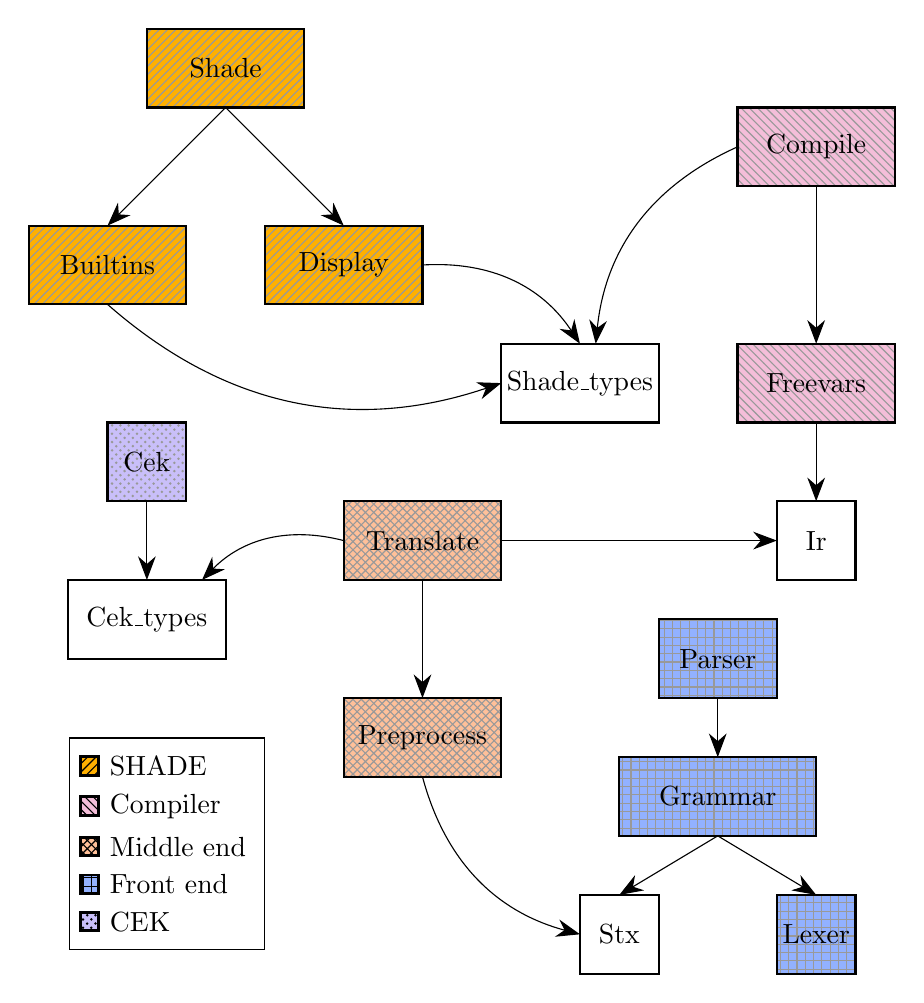
\begin{tikzpicture}[
    shadenode/.style={shape=rectangle, preaction={fill,shadecolor}, draw=black, line width=1},
    compilernode/.style={shape=rectangle, preaction={fill,compiler!30}, draw=black, line width=1},
    middlenode/.style={shape=rectangle, preaction={fill,middle!40}, draw=black, line width=1},
    frontnode/.style={shape=rectangle, preaction={fill,front!70}, draw=black, line width=1},
    ceknode/.style={shape=rectangle, preaction={fill,cek!40}, draw=black, line width=1}
]
% Grid for drafting
%\draw[step=1cm,yellow,very thin] (0,0) grid (20,20);

% Coordinates
\coordinate (stx_top) at (7.5,1);
\coordinate (stx_left) at (7,0.5);

\coordinate (lexer_top) at (10,1);

\coordinate (parser_bottom) at (8.75, 3.5);
\coordinate (grammar_top) at (8.75, 2.75);
\coordinate (grammar_bottom) at (8.75, 1.75);

\coordinate (preprocess_bottom) at (5,2.5);
\coordinate (translate_bottom) at (5, 5);
\coordinate (preprocess_top) at (5,3.5);
\coordinate (freevars_top) at (10,8);
\coordinate (compile_bottom) at (10,10);
\coordinate (cek_bottom) at (1.5,6);
\coordinate (cek_types_top) at (1.5, 5);
\coordinate (cek_types_top2) at (2.2, 5);
\coordinate (ir_top) at (10, 6);
\coordinate (ir_left) at (9.5, 5.5);
\coordinate (freevars_bottom) at (10, 7);
\coordinate (builtins_top) at (1,9.5);
\coordinate (display_top) at (4,9.5);
\coordinate (shade_types_top) at (7,8);
\coordinate (shade_types_top2) at (7.2,8);
\coordinate (shade_bottom) at (2.5, 11);
\coordinate (display_right) at (5,9);
\coordinate (compile_left) at (9,10);
\coordinate (compile_left) at (9,10.5);
\coordinate (translate_right) at (6,5.5);
\coordinate (translate_left) at (4,5.5);
\coordinate (builtins_bottom) at (1,8.5);
\coordinate (shade_types_left) at (6,7.5);

% Boxes

% middle end
\draw[middle_text, thick] (7,0) rectangle (8,1) node[pos=.5] {Stx};
\draw[middle_text, thick, preaction={fill,middle!40}, pattern=crosshatch, pattern color=szurke] (4,2.5) rectangle (6,3.5) node[pos=.5] {Preprocess};
\draw[middle_text, thick, preaction={fill,middle!40}, pattern=crosshatch, pattern color=szurke] (4,5) rectangle (6,6) node[pos=.5] {Translate};

% front end
\draw[front_text, thick, preaction={fill,front!70}, pattern=grid, pattern color=szurke] (9.5,0) rectangle (10.5,1) node[pos=.5] {Lexer};
\draw[front_text, thick, preaction={fill,front!70}, pattern=grid, pattern color=szurke] (7.5,1.75) rectangle (10,2.75) node[pos=.5] {Grammar};
\draw[front_text, thick, preaction={fill,front!70}, pattern=grid, pattern color=szurke] (8,3.5) rectangle (9.5,4.5) node[pos=.5] {Parser};

% cek
\draw[cek_text, thick] (0.5,4) rectangle (2.5,5) node[pos=.5] {Cek\_types};
\draw[cek_text, thick, preaction={fill,cek!40}, pattern=crosshatch dots, pattern color=szurke] (1,6) rectangle (2,7) node[pos=.5] {Cek};

% compiler
\draw[compiler_text, thick] (9.5,5) rectangle (10.5,6) node[pos=.5] {Ir};
\draw[compiler_text, thick, preaction={fill,compiler!30}, pattern=north west lines, pattern color=szurke] (9,7) rectangle (11,8) node[pos=.5] {Freevars};
\draw[compiler_text, thick, preaction={fill,compiler!30}, pattern=north west lines, pattern color=szurke] (9,10) rectangle (11,11) node[pos=.5] {Compile};

% shade
\draw[shade_text, thick, preaction={fill, shadecolor}, pattern=north east lines, pattern color=szurke] (0,8.5) rectangle (2,9.5) node[pos=.5] {Builtins};
\draw[shade_text, thick, preaction={fill,shadecolor}, pattern=north east lines, pattern color=szurke] (3,8.5) rectangle (5,9.5) node[pos=.5] {Display};
\draw[shade_text, thick] (6,7) rectangle (8,8) node[pos=.5] {Shade\_types};
\draw[shade_text, thick, preaction={fill=shadecolor}, pattern=north east lines, pattern color=szurke] (1.5,11) rectangle (3.5,12) node[pos=.5] {Shade};

% Arrows
\draw[-{Stealth[length=3mm]}] (preprocess_bottom) to [bend right] (stx_left);
\draw[-{Stealth[length=3mm]}] (translate_bottom) -- (preprocess_top);
\draw[-{Stealth[length=3mm]}] (compile_bottom) -- (freevars_top);
\draw[-{Stealth[length=3mm]}] (freevars_bottom) -- (ir_top);
\draw[-{Stealth[length=3mm]}] (cek_bottom) -- (cek_types_top);
\draw[-{Stealth[length=3mm]}] (shade_bottom) -- (builtins_top);
\draw[-{Stealth[length=3mm]}] (shade_bottom) -- (display_top);
\draw[-{Stealth[length=3mm]}] (display_right) to [bend left] (shade_types_top);
\draw[-{Stealth[length=3mm]}] (compile_left) to [bend right] (shade_types_top2);
\draw[-{Stealth[length=3mm]}] (translate_right) to (ir_left);
\draw[-{Stealth[length=3mm]}] (translate_left) to [bend right] (cek_types_top2);
\draw[-{Stealth[length=3mm]}] (builtins_bottom) to [bend right] (shade_types_left);

\draw[-{Stealth[length=3mm]}] (parser_bottom) to (grammar_top);
\draw[-{Stealth[length=3mm]}] (grammar_bottom) to (stx_top);
\draw[-{Stealth[length=3mm]}] (grammar_bottom) to (lexer_top);

\matrix [draw,below left] at (3,3) {
  \node [shadenode,pattern=north east lines,label=right:SHADE] {}; \\
  \node [compilernode,pattern=north west lines,label=right:Compiler] {}; \\
  \node [middlenode,pattern=crosshatch,label=right:Middle end] {}; \\
  \node [frontnode,pattern=grid,label=right:Front end] {}; \\
  \node [ceknode,pattern=crosshatch dots,label=right:CEK] {}; \\
};

\end{tikzpicture}

\end{document}
